\chapter{Evaluation}
\label{chap:evaluation}
in this chapter, we evaluate and compare various different settings

"We found crossover and mutation most influential in GA success."\cite{mills_determining_2015}

"The cross over operator is found to be the most influential parameter in both the case studies, followed by mutation rate, population size for case study-1 and population size and selection process for case study-2. It is evident that the robust GA parameter settings are sensitive"\cite{majumdar_genetic_2015}

\cite{boyabatli_parameter_2004} also suggest a high mutation rate.



It seams like the high variations does not allow for more complex traffic situations, giving a clear priority to pedestrian actions

TODO: chart: emergency break due to pedestrians vs vehicles

\section{Comparison with random and default ga Values}
scenario 1: default : 9v 5p


\begin{figure}[ht] 
	\label{figure:sim_1_comparison}
	\begin{minipage}[b]{0.5\linewidth}
		\centering
		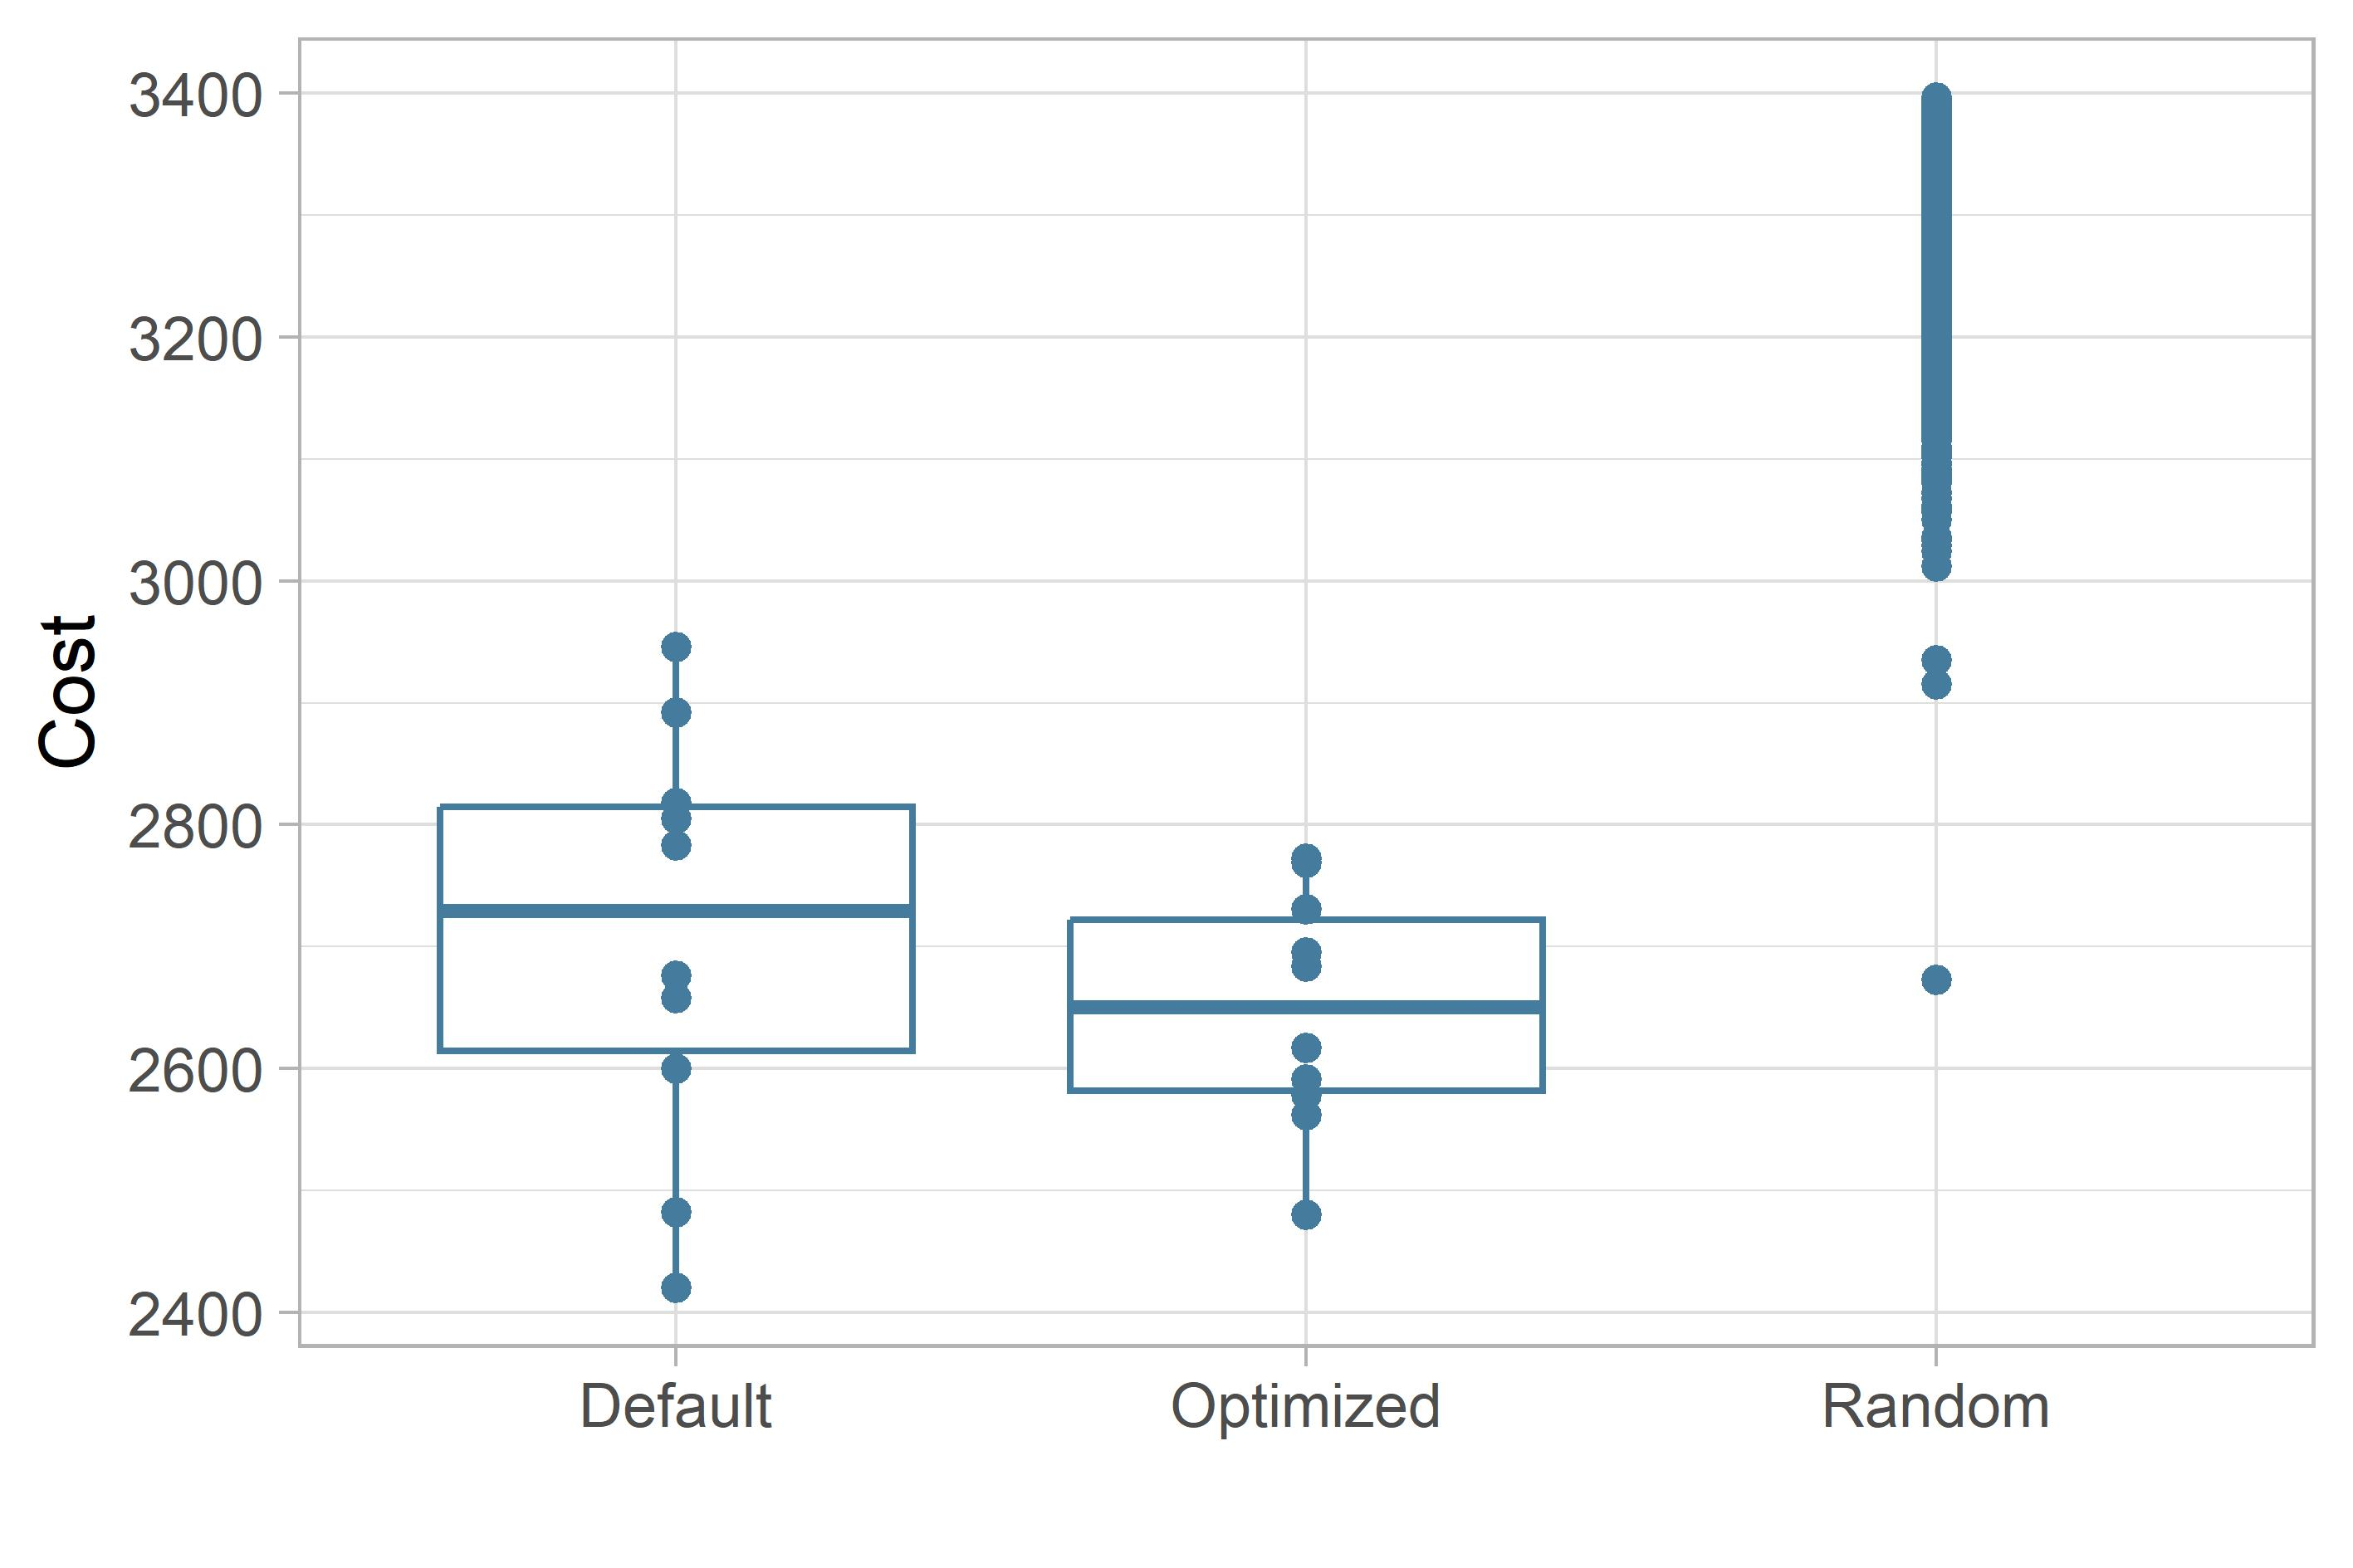
\includegraphics[width=1\linewidth]{simulations/evaluation/plots/sim_1_comparison} 
	\end{minipage}%%
	\begin{minipage}[b]{0.5\linewidth}
		\centering
		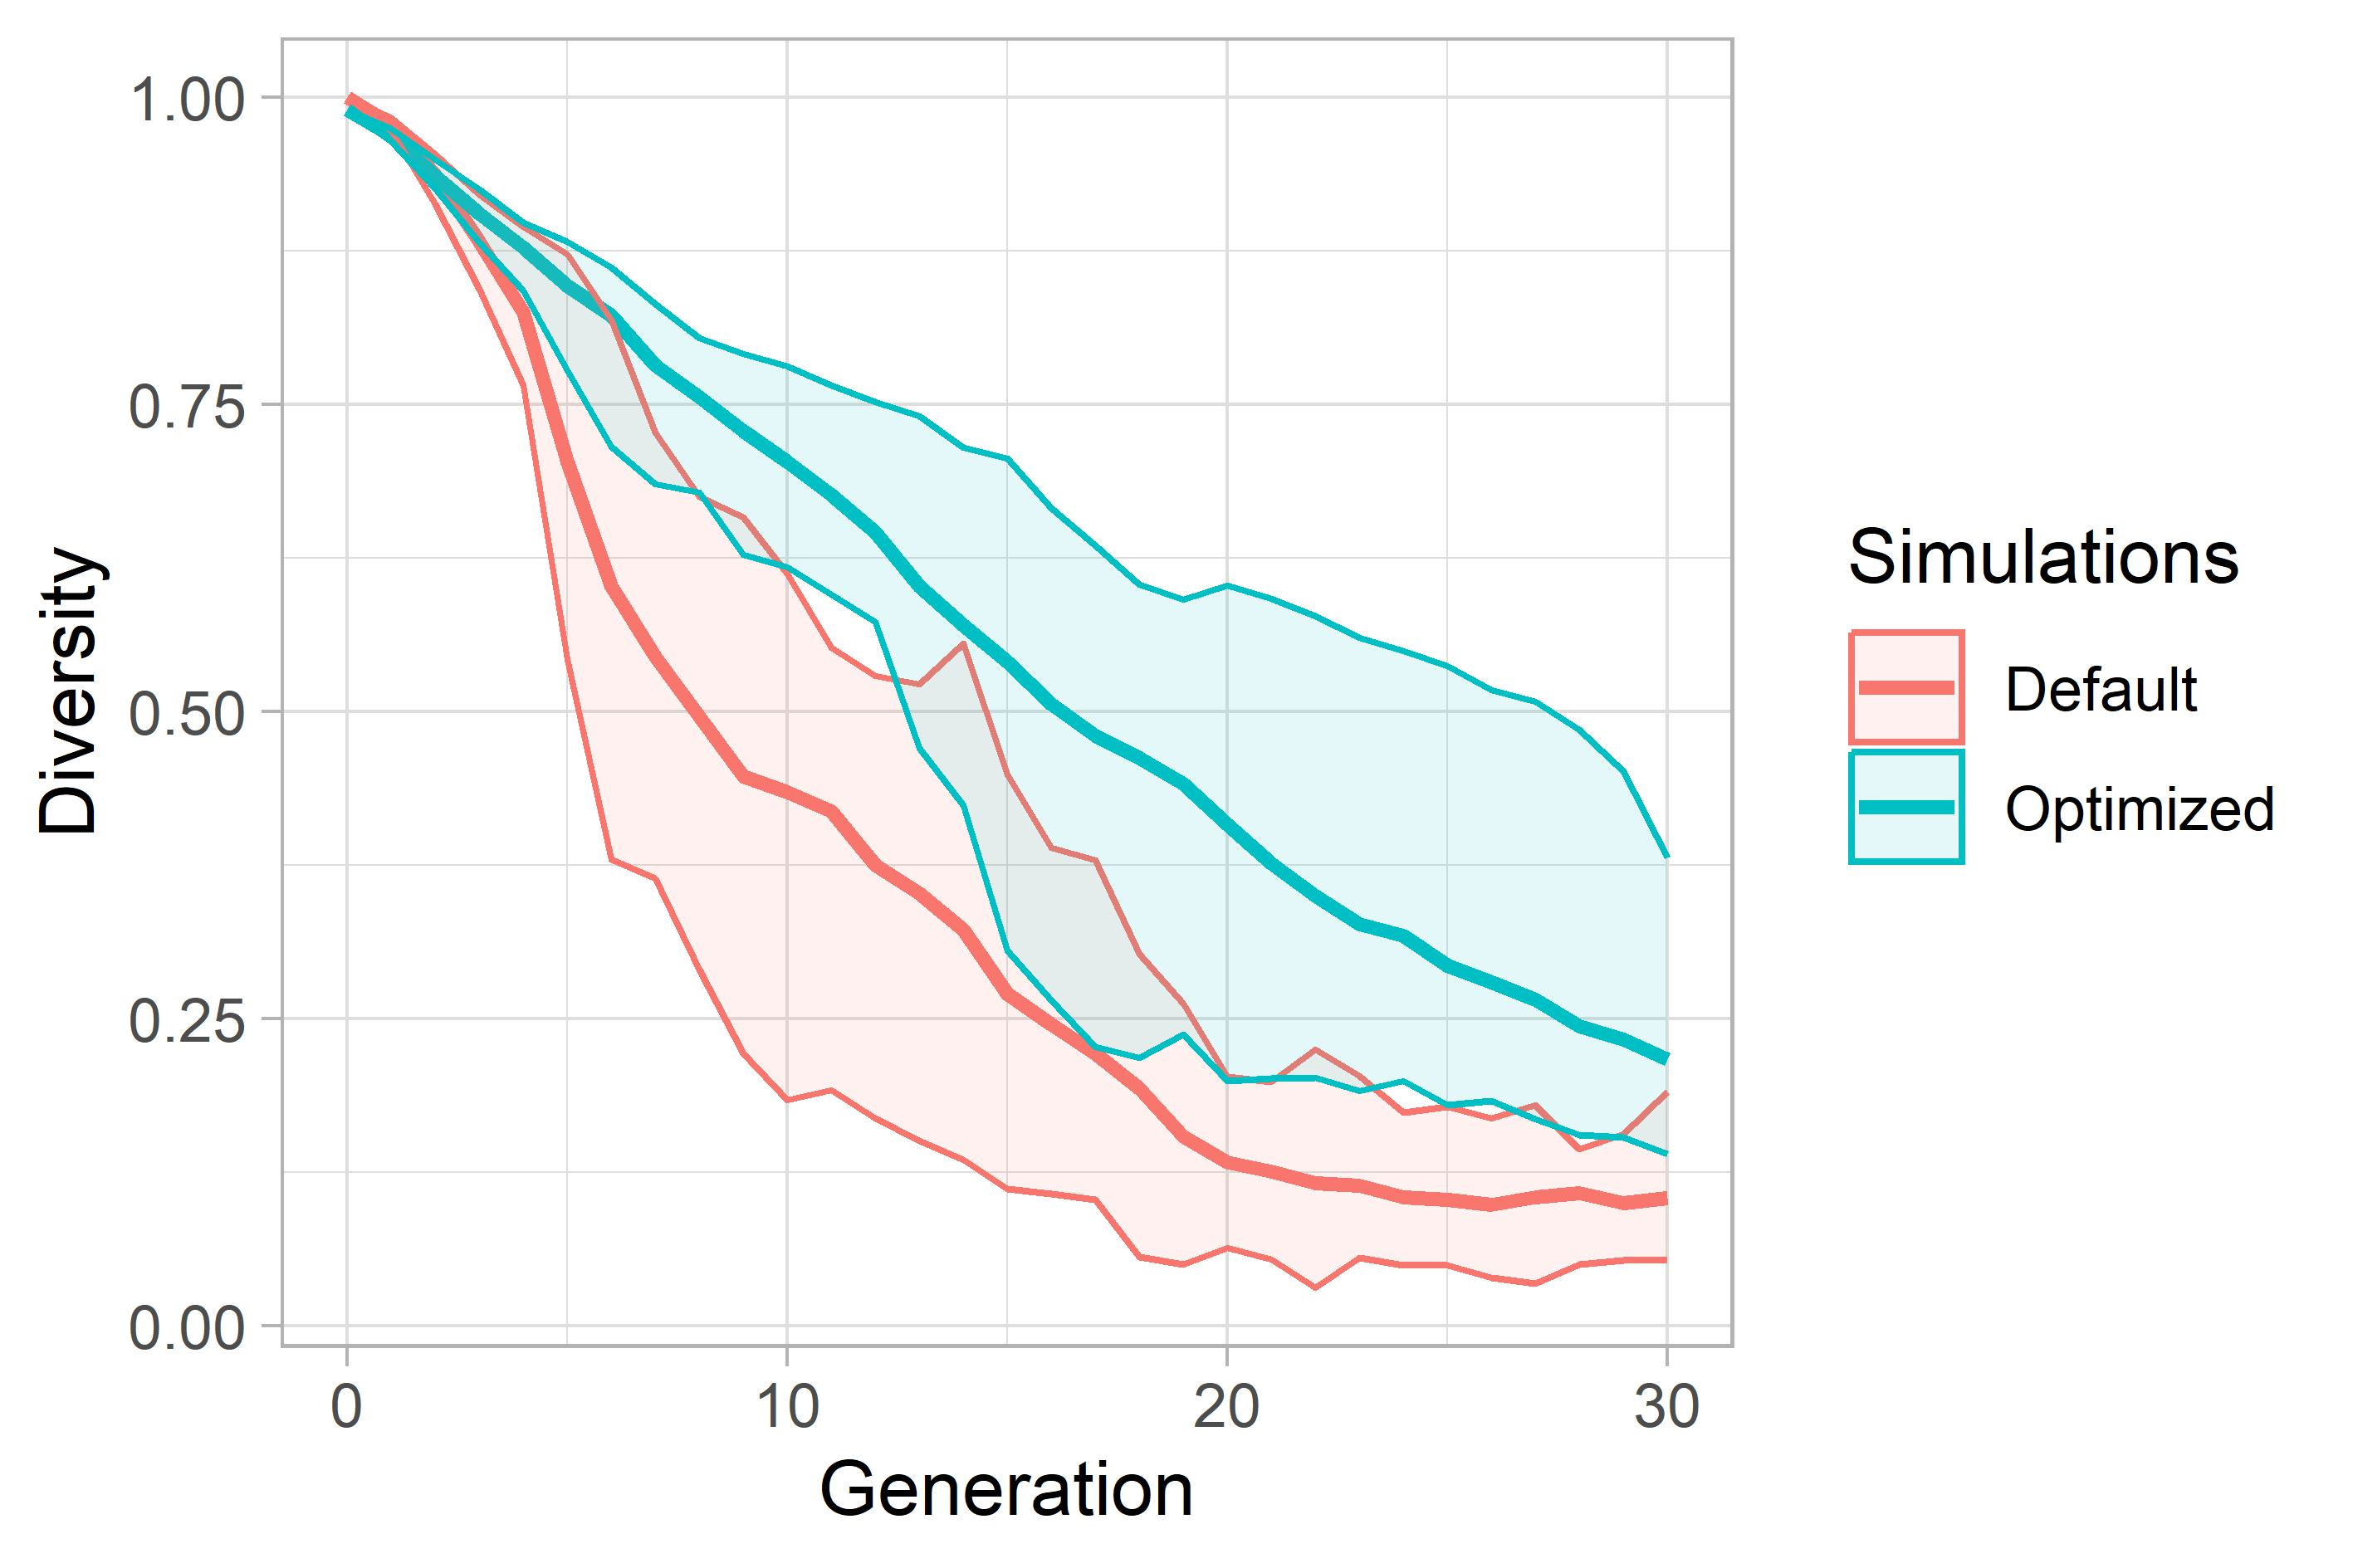
\includegraphics[width=1\linewidth]{simulations/evaluation/plots/sim_1_diversity} 
	\end{minipage} 
	\caption{Comparison Simulation 1: Default GA vs Optimized GA vs Random}
\end{figure}


\section{Generalization on different start scenarios}

\subsubsection{Scenario 2}
scenario 2: 9v 5p
\begin{figure}[ht] 
	\label{figure:sim_2_comparison}
	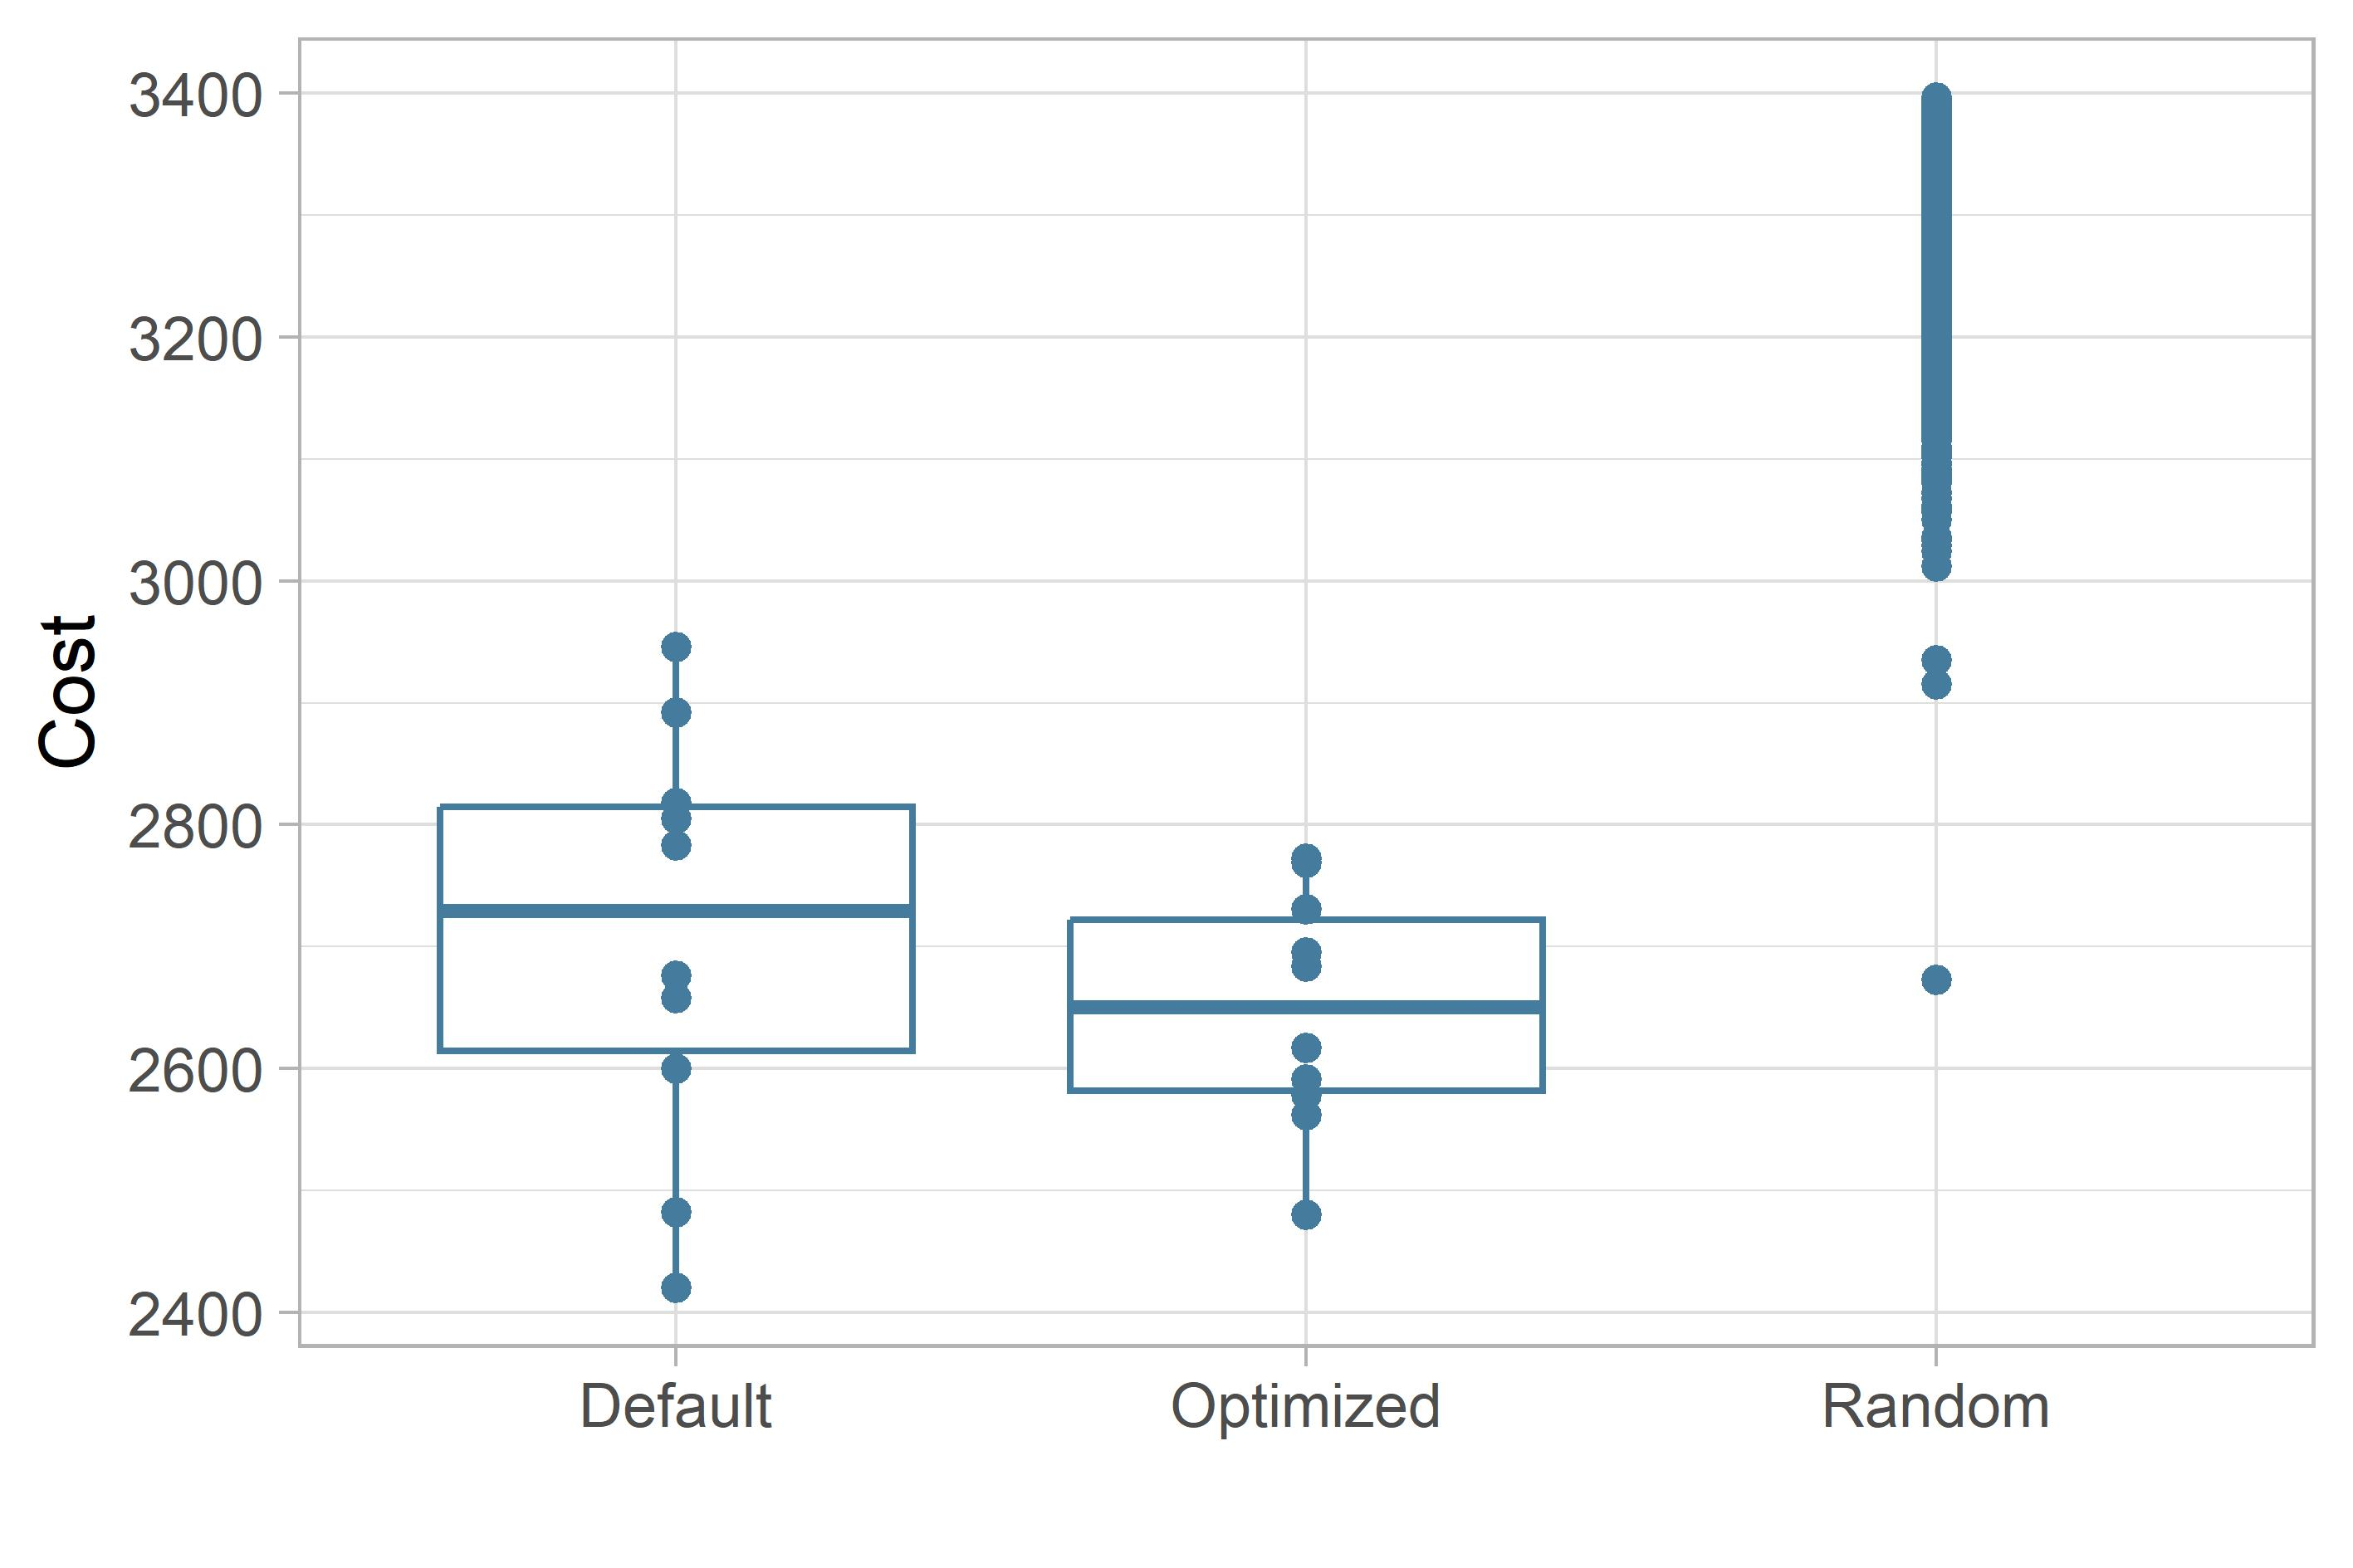
\includegraphics[width=1\linewidth]{simulations/evaluation/plots/sim_1_comparison}
	\caption{Genetic Algorithm with Elite}
\end{figure}


\subsubsection{Scenario 3}
scenario 3: 5v 3p
\begin{figure}[ht] 
	\label{figure:sim_3_comparison}
	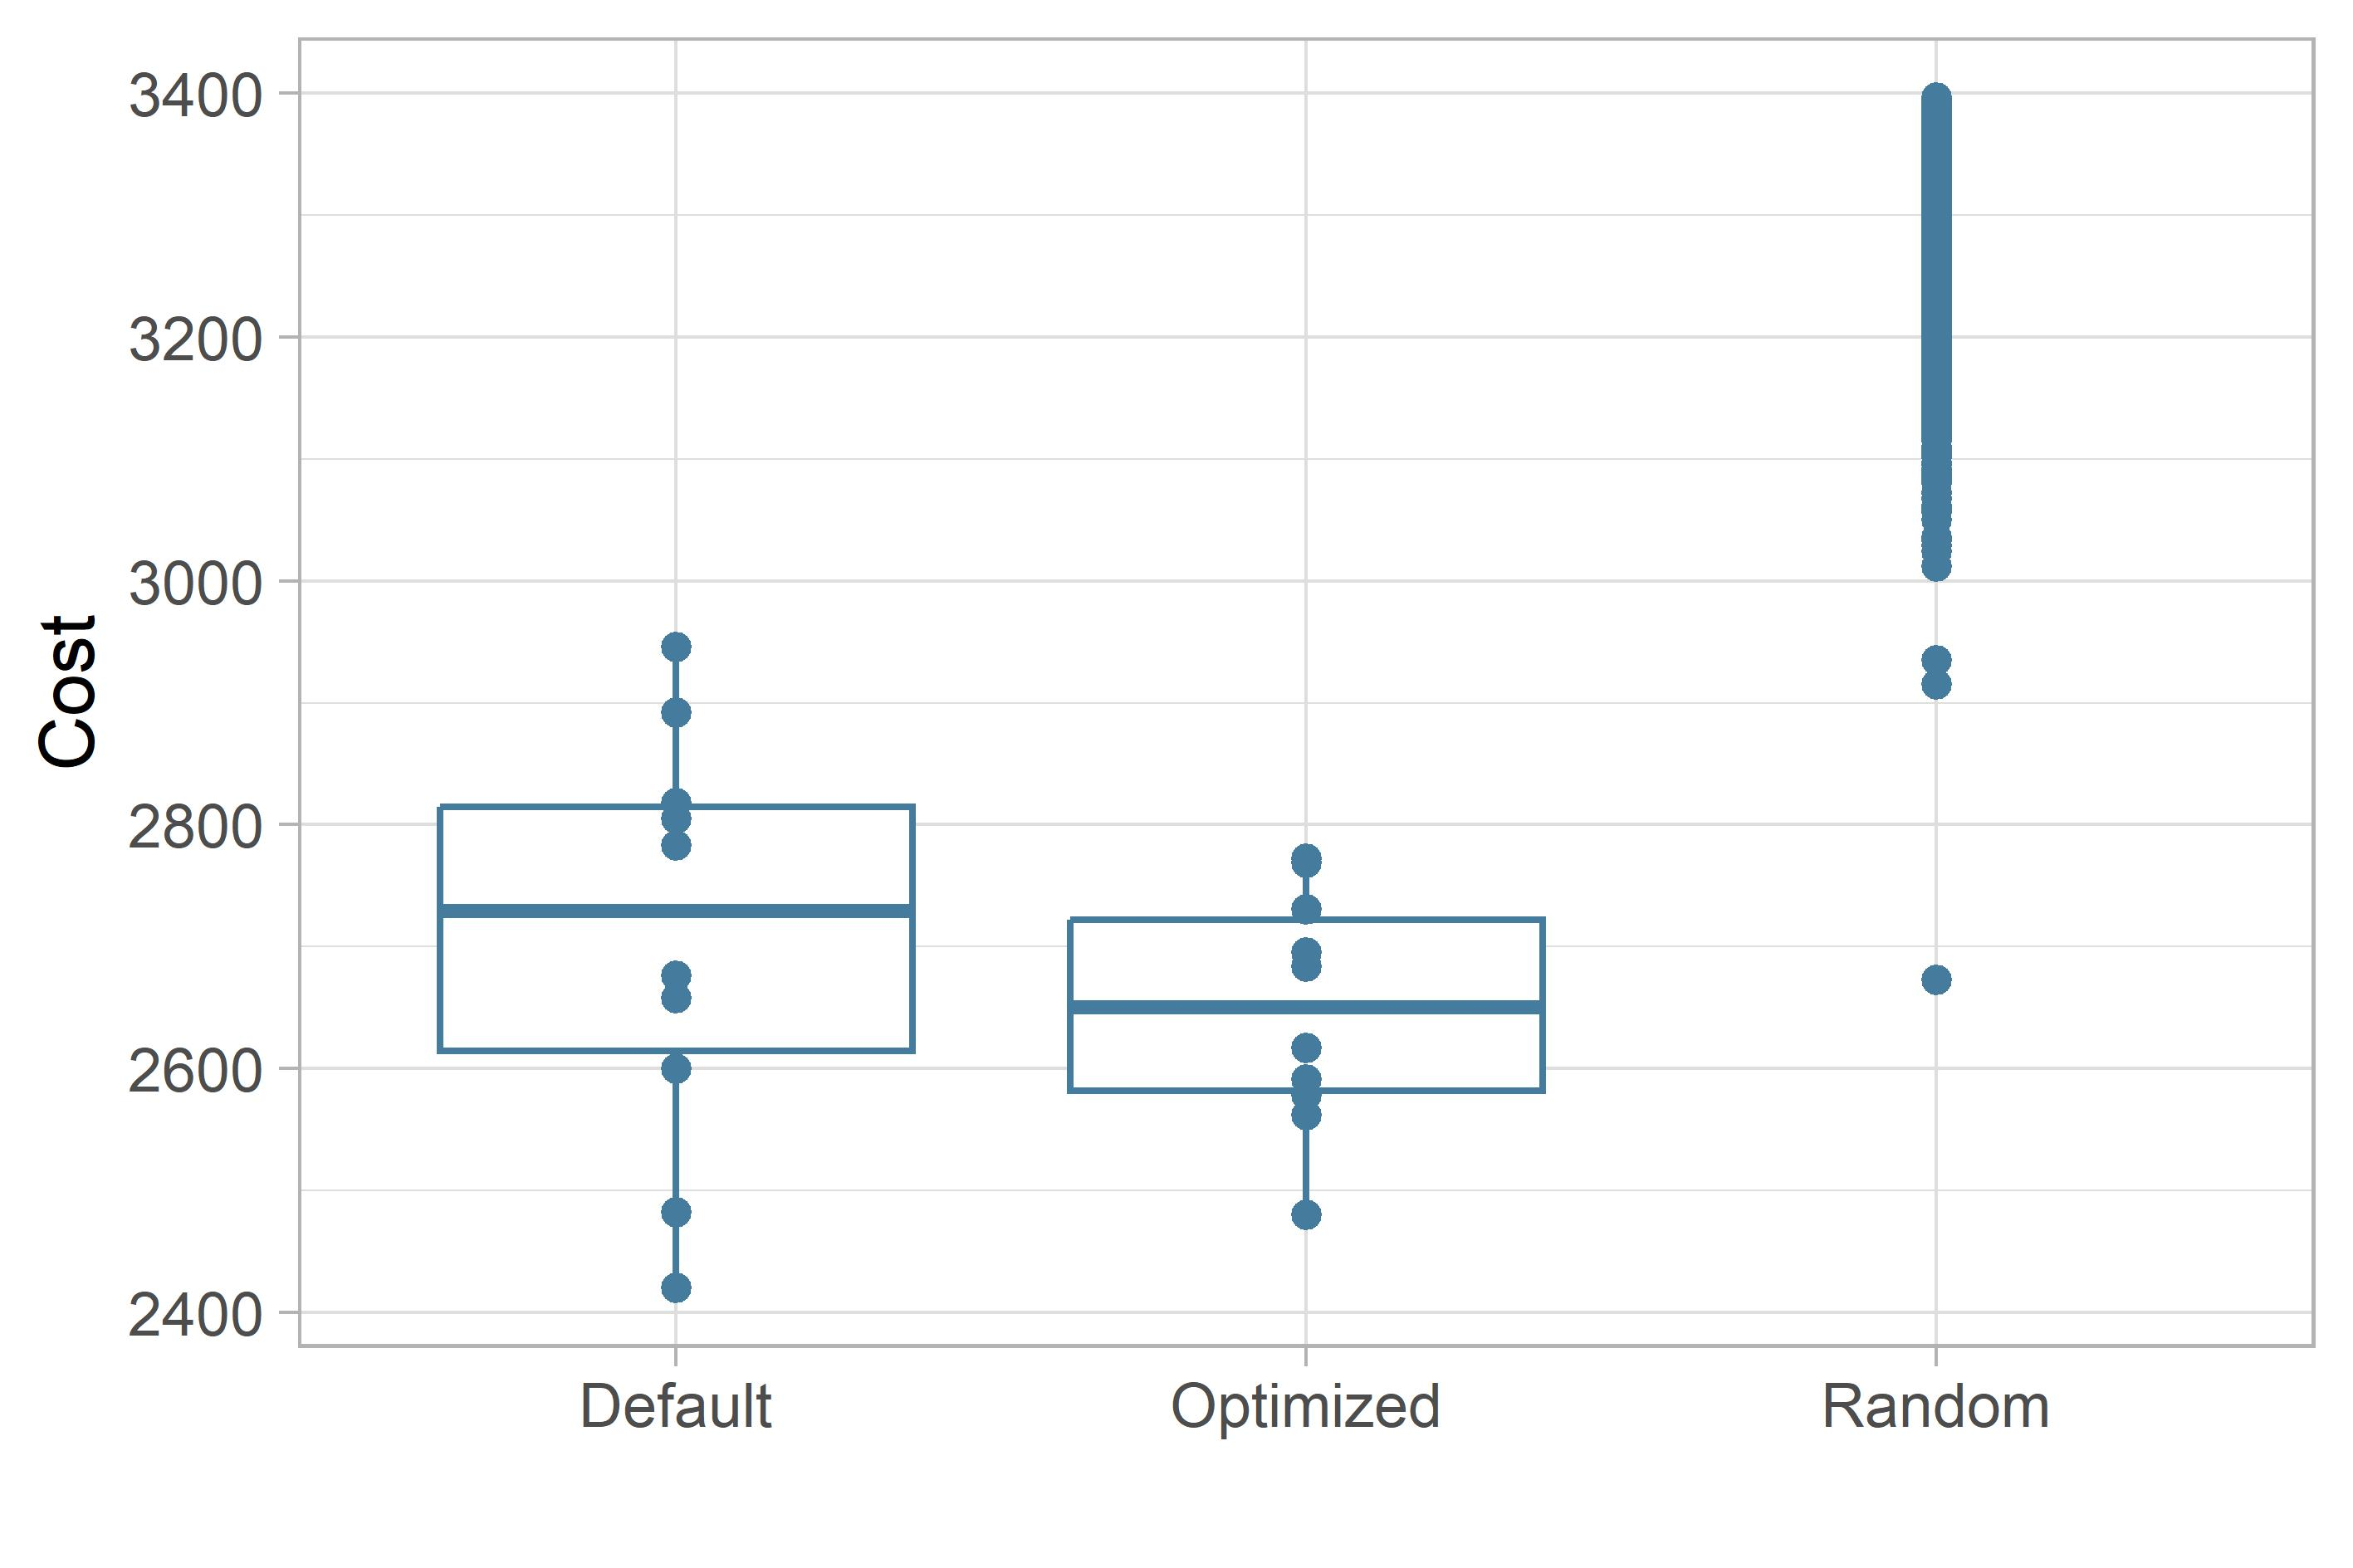
\includegraphics[width=1\linewidth]{simulations/evaluation/plots/sim_1_comparison}
	\caption{Genetic Algorithm with Elite}
\end{figure}

\subsubsection{Scenario 4}
scenario 4: 18v 10p
\begin{figure}[ht] 
	\label{figure:sim_4_comparison}
	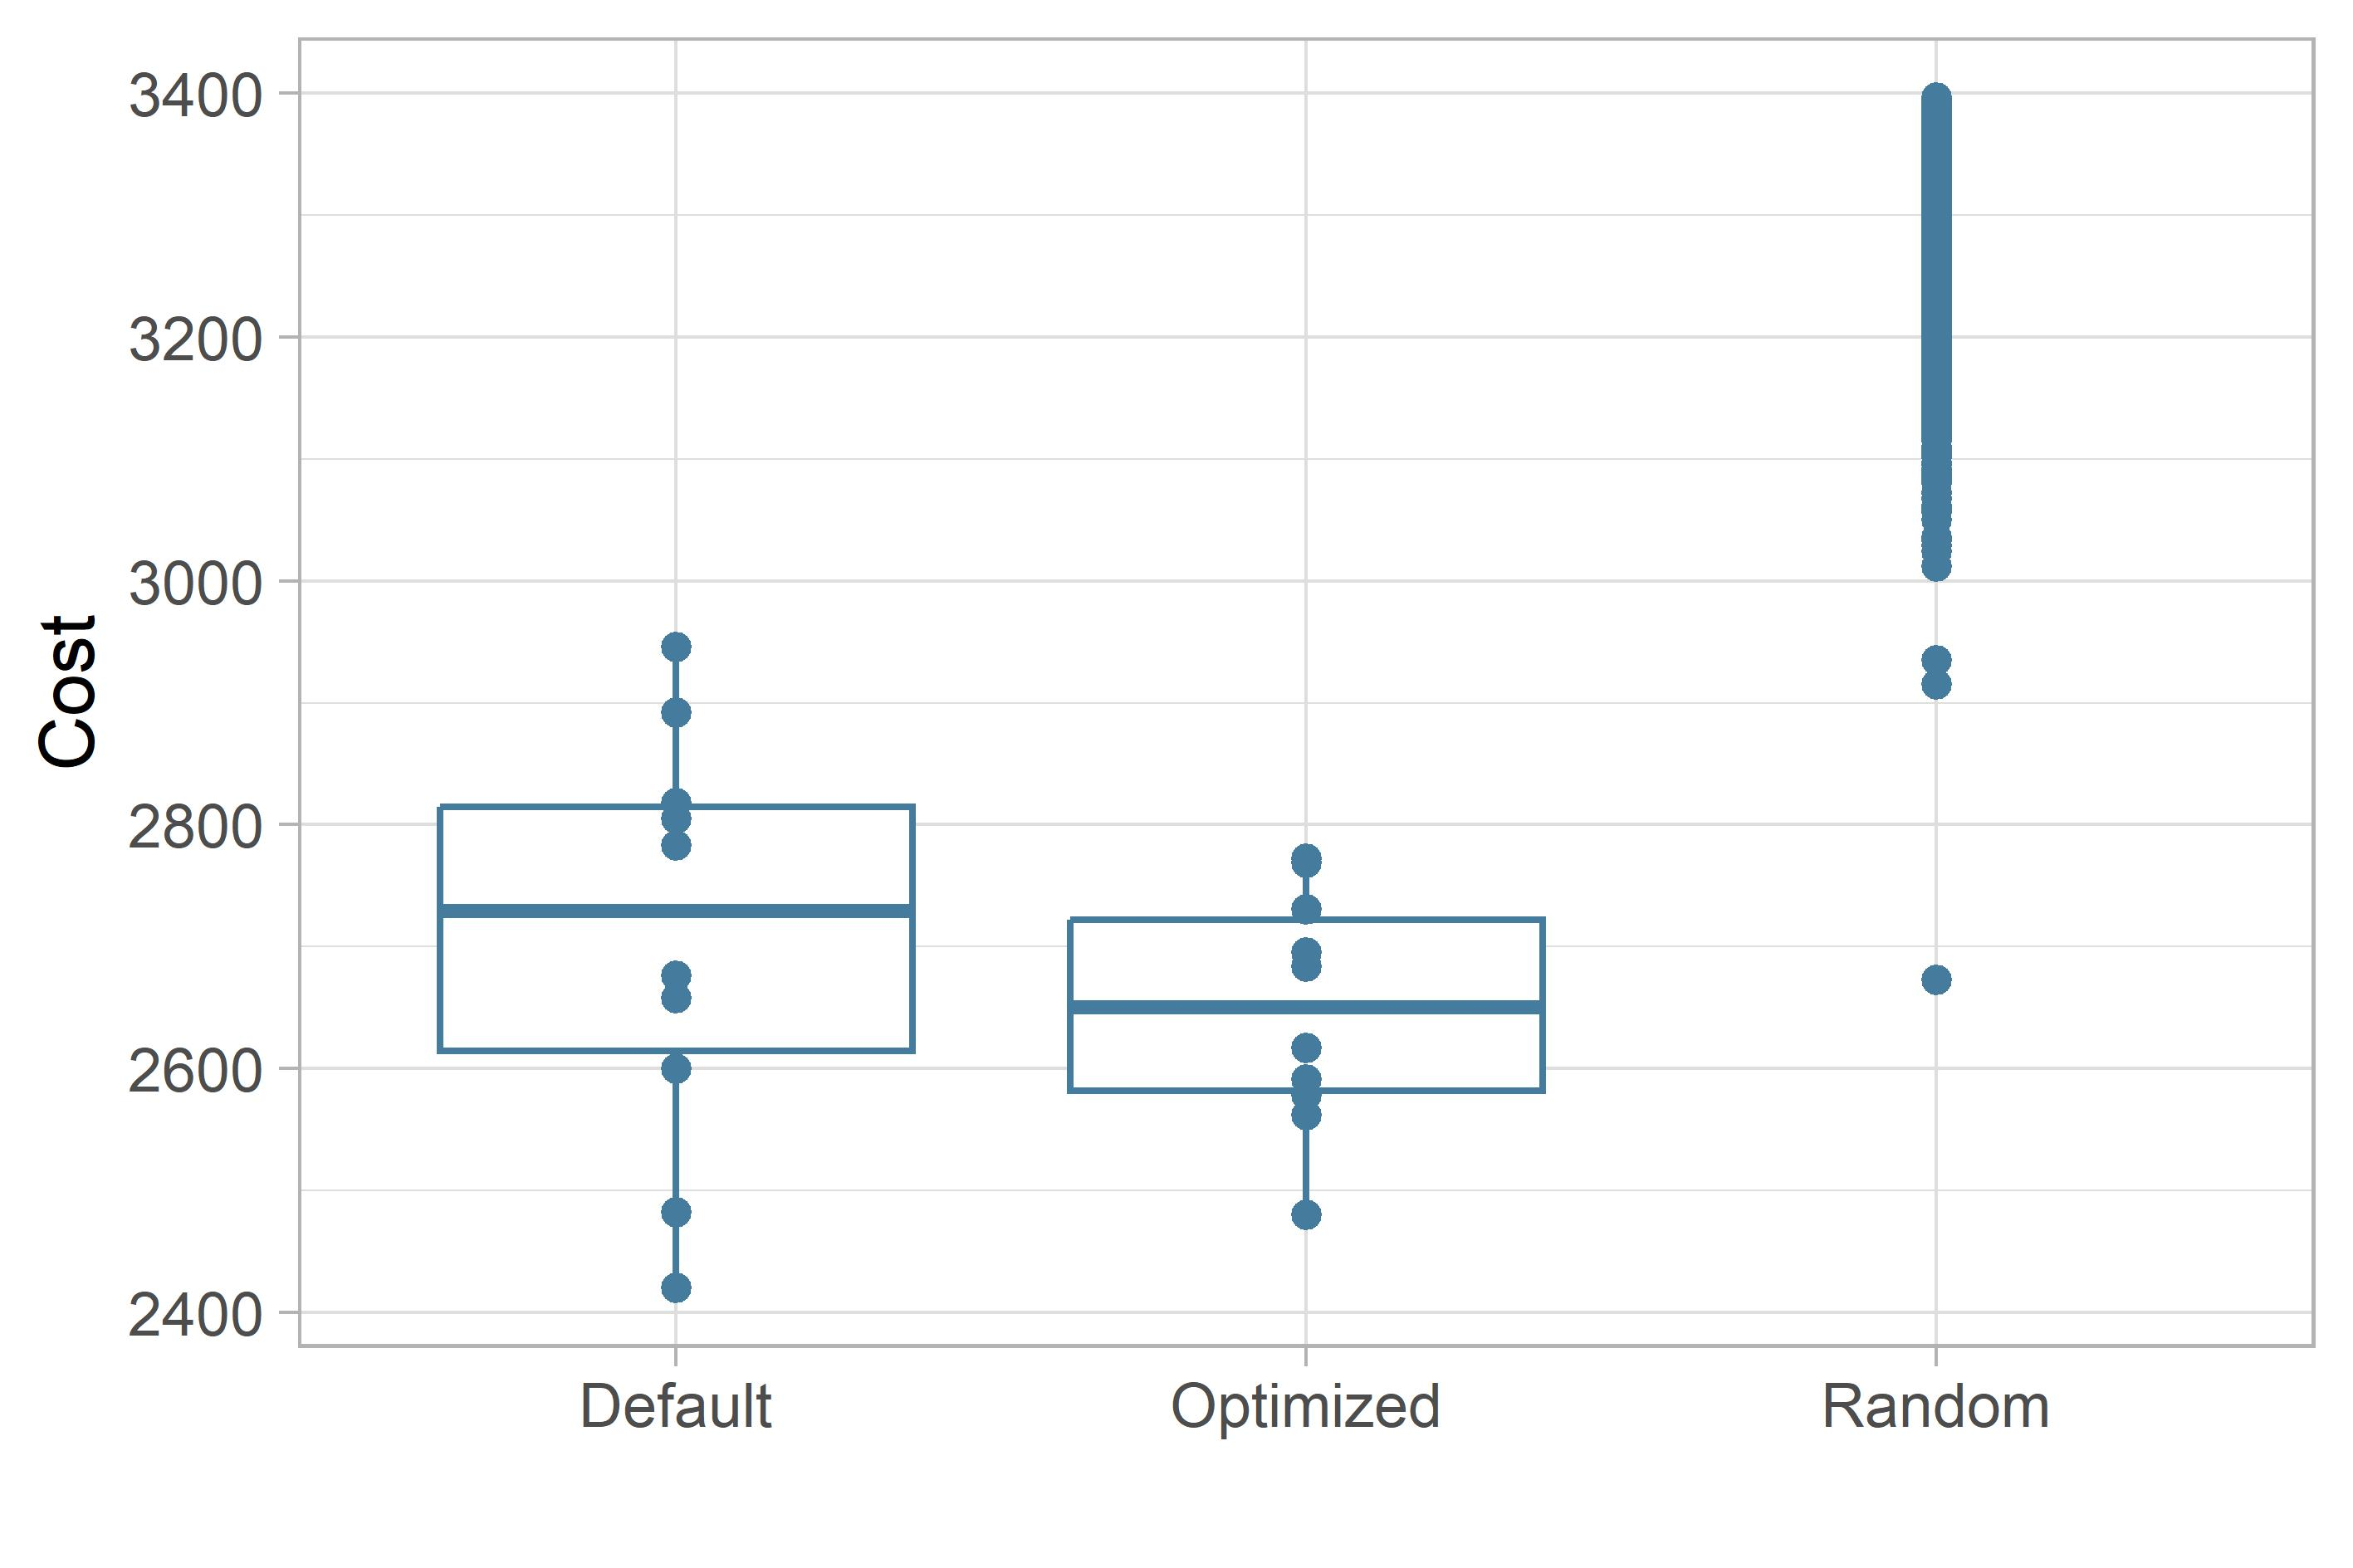
\includegraphics[width=1\linewidth]{simulations/evaluation/plots/sim_1_comparison}
	\caption{Genetic Algorithm with Elite}
\end{figure}



\todo{also compare (average) diversity?}